\documentclass[main.tex]{subfiles}

\begin{document}

	\begingroup

	\renewcommand{\cleardoublepage}{}

	\renewcommand{\clearpage}{}

	\chapter{Knowledge Function Documentation}

		\chapterauthor{Jeremias Thun}

All the Information about the existing surfaces and the objects are managed in our Knowledgebase. Every question about the relationship between these Objects as well as which ones should be taken next and where it should be put is answered by this Knowledgebase.  The Knowledgebase is built as part of \textit{KnowRob}. All data is stored as \textit{RDF triple}, organized by an OWL ontology. This is where the logical relationship between the category of objects and surfaces is implemented.

Most of the Knowledge part is based on the knowledge processing system \textit{KnowRob} (www.knowrob.org), which provides us with the fundamental opportunity to not only work with \textit{Prolog} in ROS and organize our Knowledge in \textit{RDF triples} based on ontologies that themselves are also based on \textit{KnowRob}, it also provides a lot of fundamental and utility functions to make storing and processing all the knowledge easier. 
		
\section{Knowledge base}
\chapterauthor{Jeremias Thun}

The Knowledgebase as well as \textit{KnowRob} is written in \textit{Prolog}. To interact manually with the Knowledgebase, you can (after you started Knowledge) run
\begin{lstlisting}
rosrun rosprolog rosprolog_commandline.py
\end{lstlisting}
which opens a \textit{Prolog} shell in your command line.

\subsection{object\_state.pl}

First of all, we need to add some objects that we can work on to our Knowledgebase. This is where the perceived objects go when the Perception-Group found something:

\begin{lstlisting}
create_object_at(
	PerceivedObjectType, 
	PercTypeConfidence, 
	Transform, 
	Threshold, 
	Instance, 
	[Width, Depth, Height], 
	Shape, 
	PercShapeConfidence, 
	Color, 
	PercColorCondidence) :-
\end{lstlisting}
This confusingly big predicate takes all the perceived Data, creates a corresponding Object in the Knowledgebase, and adds all the attributes. Within this procedure, there are a few verifications and changes made, though: The Class, Shape, and Color of the Object all have a probability with which they are correctly perceived. These confidences are stored as a link to the Object (more on that in the OWL-Chapter), but only if they satisfy a specified threshold. If they don't, the attributes are set back to default values. Also, we check if the given data makes any sense, i.e. if the object has a reasonable size.\\
Besides a few helper predicates, this module also contains two helpful little predicates to get all Objects that are stored at that moment:
\begin{lstlisting}
hsr_existing_objects(Objects) :-
    belief_existing_objects(Objects, [hsr_objects:'Item']).
\end{lstlisting}
And there \textit{hsr\_forget\_object/1} removes an Object from the beliefstate:
\begin{lstlisting}
hsr_forget_object(Object) :-
    rdf_retractall(Object,_,_).
\end{lstlisting}

\subsection{beliefstate.pl}

In the Belief State mostly all changing information about our Knowledge is managed. Here lie the predicates that are called in \textit{create\_object\_at/9}. To create a new Object in our belief state, there is:
\begin{lstlisting}
new_perceived_at(ObjType, Transform, Threshold, Instance) :-
\begin{lstlisting}
This Module also allows looking at a specific position in the map and ask, whether there already is a known Object and, if so, which one:
\begin{lstlisting}
hsr_existing_object_at(_, Transform, Threshold, Instance) :-
\end{lstlisting}
To determine, whether an object is hard to grasp it is often helpful to know, whether there are other objects right next to it. That is why there is a specific attribute that stores Groups of Objects. 
\begin{lstlisting}
group_objects(Objs)
\end{lstlisting}
This Predicate takes a list of Objects and iterates through them to see if there are any groups and create them if necessary.\\
To make it more human-readable, there are also two other predicates that basically just call \textit{group\_objects} with a different list of Objects:
\begin{lstlisting}
group_shelf_objects/0
group_table_objects/0
\end{lstlisting}

\subsubsection{Finding a goal surface for an Object\label{sec:kn_find_surf}}

The second part of our beliefstate decides, what surface Knowledge beliefs to be the best fit for an object at a certain time. This part still has a few flaws but here is what it does:
\begin{figure}
\centering
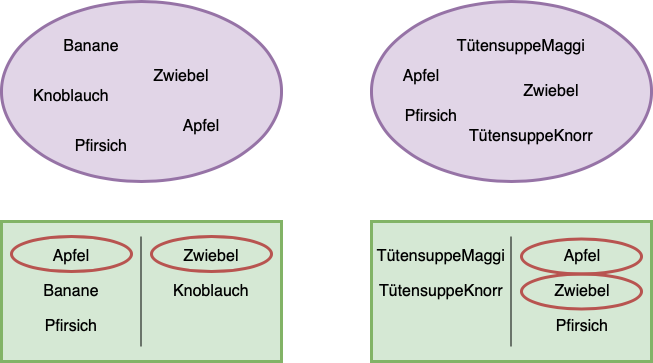
\includegraphics[width=0.8\textwidth]{pictures/knowledge/knowledge_placing_objects}
\caption{The object placing strategy}
\label{fig:kn_obj_placement}
\end{figure}

Based on all the known objects, we want to find a suitable grouping on the shelf floors for them. This grouping needs to be more detailed if the known objects are more similar and it needs to be less specific if we have a wider range of very different objects (as you can see in figure \ref{fig:kn_obj_placement}). On the other hand, we need to stay flexible in case we haven't scanned the whole scene at this point or if the scene changes behind our back. For example, if the second scene in figure \ref{fig:kn_obj_placement} finds another Apple and a Banana later, Knowledge should reconsider the earlier grouping and maybe open a third floor.

This is achieved by first taking the one object we want to place right now and finding the object that is most similar to it, standing on a target surface. The predicate
\begin{lstlisting}
most_related_object(Source, Target) :-
\end{lstlisting}
first looks for objects with a similar class and finds the logical distance to that class. If that distance is below a threshold defined in \textit{config.pl} and that class is not the general fallback \textit{hsr\_objects:'Other'}, this most related object gets linked to the first object as it's \textit{refObject} and the first object also gets the distance stored.\\
If the criteria don't match, \textit{most\_related\_object} looks for a suitable object with a similar color or size instead and otherwise does the same procedure. The distance is defined as always a bit more than the maximum class difference, so sorting by class is always preferred.

Once the reference object is found, the supposed surface seems to be the one, that reference object is standing on. But what if we just assigned an onion to an apple, while we already know about two bananas and a peach, that would fit much better to that apple? To avoid that, we are now running the \textit{most\_related\_object/2} for all the other known objects on \textit{source} surfaces and take the ones, that should end up on the same surface as our first object. This is done by the predicate
\begin{lstlisting}
% OtherObjects returns a list of all the objects, that one day 
% would be put on Surface.
objects_on_same_surface_in_future(Surface, OtherObjects) :-
\end{lstlisting}
which also sorts all the objects that should end up on that surface by the "distance" to their \textit{refObject}. This way, the objects that come first in the list \textit{OtherObjects} are more similar to one of the objects already placed on that surface than the ones that come later in the list.

Based on that list it is pretty easy, to just add up the width of the first few objects and cut the list where the objects don't fit on their \textit{supposedSurface} anymore, which is done by the predicate
\begin{lstlisting}
% Takes a list of objects and divides it into the first n objects that fit on
% the given surface and the rest.
objects_fit_on_surface(Objects, Surface, FittingObjects, NotFittingObjects) :-
\end{lstlisting}

In the end, all the \textit{FittingObjects} have found their \textit{supposedSurface}. This surface is now stored as an RDF link to them so we don't need to restart the whole calculation every time we want to place one of them. The other \textit{NotFittingObjects}, as well as all the objects supposed to go on a different surface, are now without a proper surface though. If one of them needs to be placed, the whole procedure would start again. If in the meantime we found some other objects that would fit better on a surface some objects are already assigned to, these assignments can be removed to make space for the new better fitting objects. All of this is organized by the predicate 
\begin{lstlisting}
object_goal_surface_(Object, Surface, Context, RefObject) :-
\end{lstlisting}

\subsection{pickup.pl}\label{sec:kn_pickup}

In the pickup module the information necessary to pick an object up are organized.

\begin{lstlisting}
next_object_(BestObj) :-
\end{lstlisting}
As soon as there are some objects stored in our belief state, Knowledge can tell, which Object should be the next one, the robot takes and puts somewhere. This predicate returns the Object, that is standing on a surface, that was previously declared as \textit{source} surface and is closest to the robot.

\subsection{assignplaces.pl}

Like \textit{pickup.pl}, this module organizes the information necessary for when an object is placed.\\

In the end, everything Planning needs is given by
\begin{lstlisting}
object_goal_pose_offset_(Instance, [[X,Y,Z], Rotation],Context):-
\end{lstlisting}
It takes an Object and returns the pose this object should be placed in and as Context, it also returns, why this decision was made the way it was.\\
It looks for the \textit{object\_goal\_surface/4} (see section \ref{fig:kn_obj_placement} under 'Finding a goal surface for an Object') and finds a suitable position for the object on that surface. To do that, it adds an offset to the position of the \textit{refObject} and returns that position in the world frame.

\subsection{surfaces.pl}

The biggest module is the \textit{surfaces} module. This is where you can find everything you need to know about surfaces.\\
The surfaces are, just like objects, stored as an atom, which represents an instance of an OWL-Class and looks like this:
\begin{lstlisting}
?- is_surface('http://ontologydesignpatterns.org/ont/dul/DUL.owl#PhysicalObject_UHOJSVEC')
true.
\end{lstlisting}
The only exception is the surface \textit{ground}, which has no representation in the URDF and is just an infinite surface that is everywhere below a certain height. This surface is just stored like this:
\begin{lstlisting}
?- is_surface(ground)
true.
\end{lstlisting}

Right now, Knowledge can handle four different types of surfaces: Tables, Shelves, Buckets, and the Ground, as you can see in the figures \ref{fig:kn_first_surface} to \ref{fig:kn_last_surface}. They are not limited in number, but it would take some rewriting in the URDF script to work with different \textit{types} of surfaces.

\begin{figure}
\label{fig:kn_surfaces}
    \centering
    \begin{minipage}{0.45\textwidth}
        \centering
        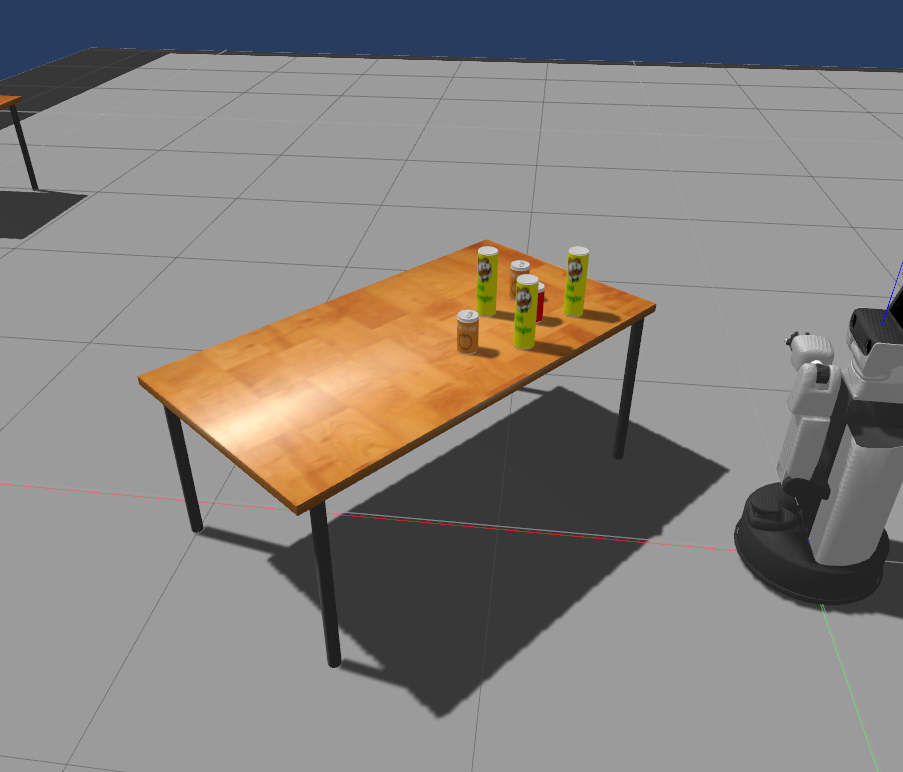
\includegraphics[width=0.95\textwidth]{pictures/knowledge/table}
        \caption{The Table surface}
        \label{fig:kn_first_surface}
    \end{minipage}\hfill
    \begin{minipage}{0.48\textwidth}
        \centering
        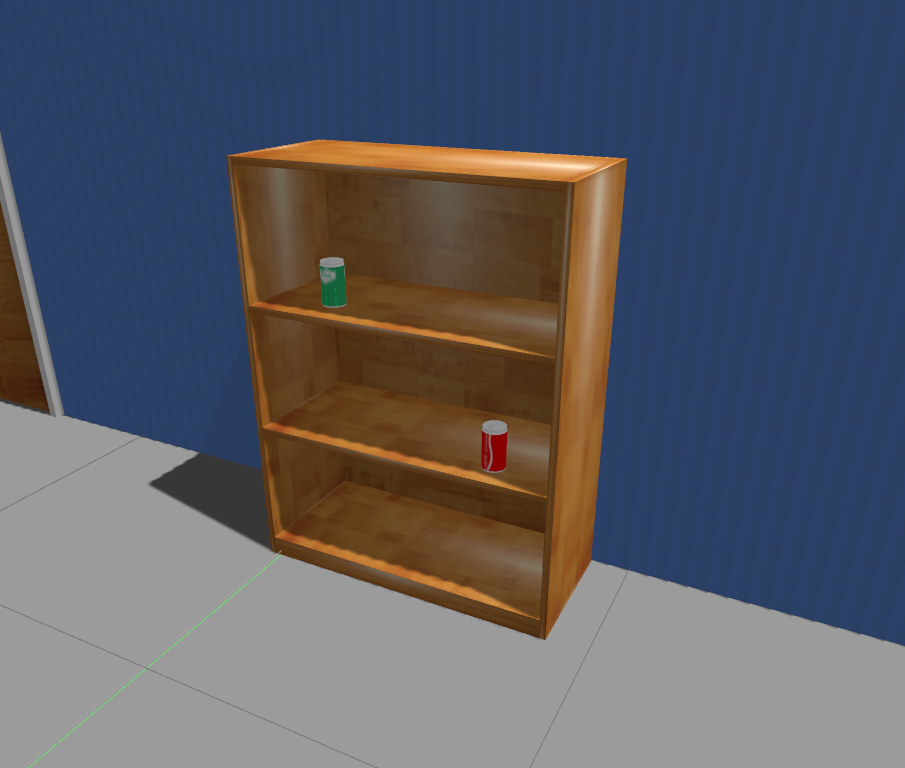
\includegraphics[width=0.95\textwidth]{pictures/knowledge/shelf}
        \caption{The Shelf surface}
        \label{fig:kn_ro_cl}
    \end{minipage}\\
    ~\\
    \begin{minipage}{0.45\textwidth}
        \centering
        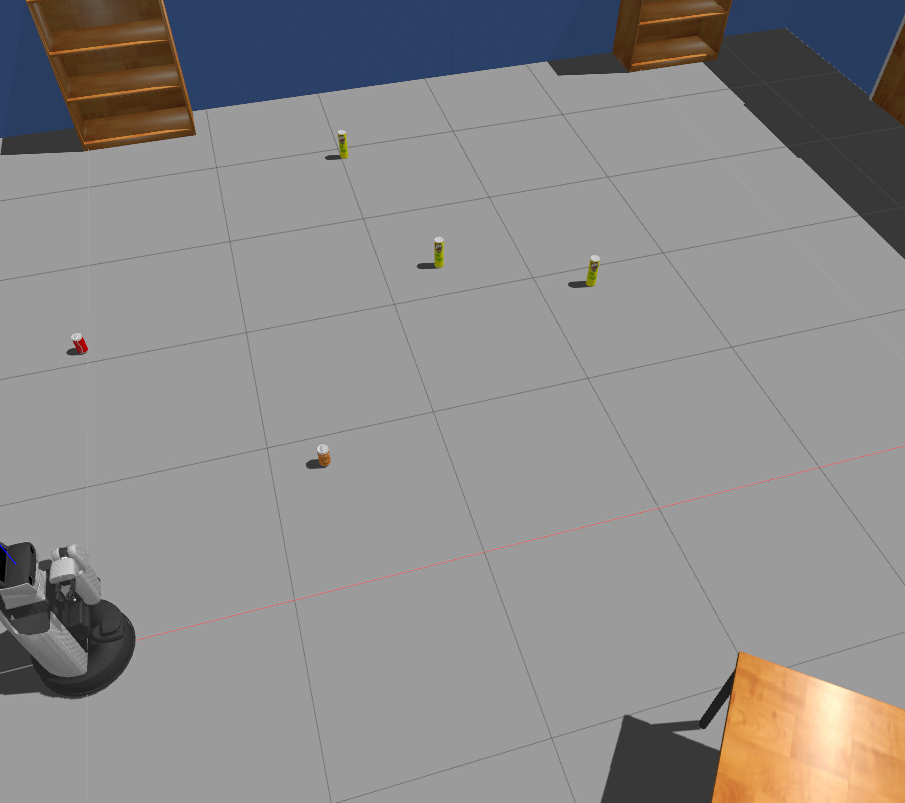
\includegraphics[width=0.95\textwidth]{pictures/knowledge/ground}
        \caption{The Ground surface}
        
    \end{minipage}\hfill
    \begin{minipage}{0.48\textwidth}
        \centering
        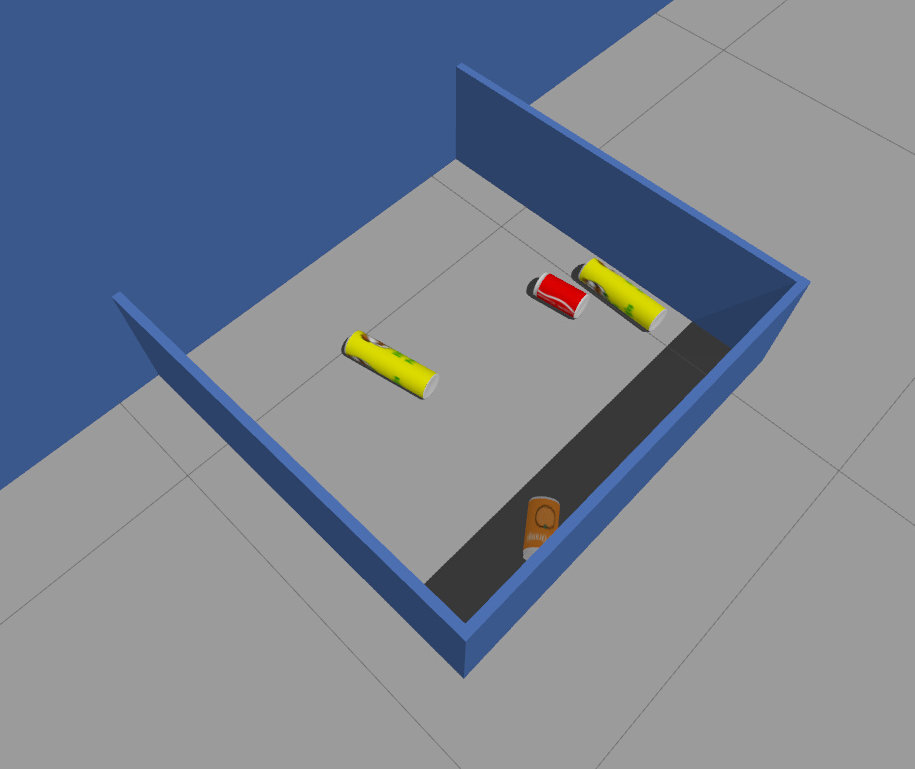
\includegraphics[width=0.95\textwidth]{pictures/knowledge/bucket}
        \caption{The Bucket surface}
        \label{fig:kn_last_surface}
    \end{minipage}
\end{figure}

\subsubsection{Find surfaces}

You can call
\begin{lstlisting}
all_surfaces/1
\end{lstlisting}
to get all surfaces that are loaded in the URDF regardless of their role or if they even have a role. This predicate comes in handy if you want to iterate through the available surfaces.\\
To find surfaces of a specific type, there are equivalent predicates that can give you lists of all tables, shelves, the ground or all source or target surfaces:
\begin{lstlisting}
all_source_surfaces/1
all_target_surfaces/1
ground_surface/1
shelf_surfaces/1
table_surfaces/1
\end{lstlisting}

There are also a few predicates that go in the other direction: If you have a surface and want to know if it is of a certain type, you can execute one of the following predicates:
\begin{lstlisting}
surface_type_of(Surface, Type) :-

is_surface(Surface) :-
    all_surfaces(Surfaces),
    member(Surface, Surfaces).

is_table(Table) :-
    table_surfaces(Tables),
    member(Table, Tables).

is_shelf(Shelf) :-
    shelf_surfaces(Shelves),
    member(Shelf, Shelves).
\end{lstlisting}
\textit{surface\_type\_of/2} expects returns the type as simple atom, which can be \textit{ground}, \textit{table} or \textit{shelf}.\\
Last but not least there is 
\begin{lstlisting}
find_supporting_surface/2
\end{lstlisting}
which goes in both directions and links an object to the surface it is standing on.

\subsubsection{Get poses}
When the Roboter first goes to a surface to scan the objects that are standing there, Planning needs to know the positions of those surfaces. That's what this chapter is about. It is based on
\begin{lstlisting}
pose_of_surfaces(Surfaces, Positions) :-
\end{lstlisting}
which takes a list of surfaces, sorts them by their distance to the robot (where the nearest surface comes first in the list) and returns the sorted list of their positions.\\
The two other predicates just call \textit{pose\_of\_surfaces/2} with a preset list of surfaces of a specified type:
\begin{lstlisting}
pose_of_tables(Positions) :-
pose_of_shelves(Positions) :-
\end{lstlisting}

\subsubsection{Find Objects}
As an equivilant to \textit{is\_surface} we also have
\begin{lstlisting}
is_object/1
\end{lstlisting}
To find Objects, there is our core predicate
\begin{lstlisting}
objects_on_list_of_surfaces(ObjectInstances, SurfaceList):-
\end{lstlisting}
which just runs through all the given surfaces and returns a list of every object that was found on them.\\
All the other predicates in this chapter are variations of this idea:
\begin{lstlisting}
objects_on_surface/2,
all_objects_on_source_surfaces/1,
all_objects_on_target_surfaces/1,
all_objects_on_ground/1,
all_objects_in_whole_shelf_/1,
all_objects_on_tables_/1,
\end{lstlisting}

\subsubsection{Roles}

\begin{figure}
    \centering
    %\begin{minipage}{0.45\textwidth}
    %    \centering
        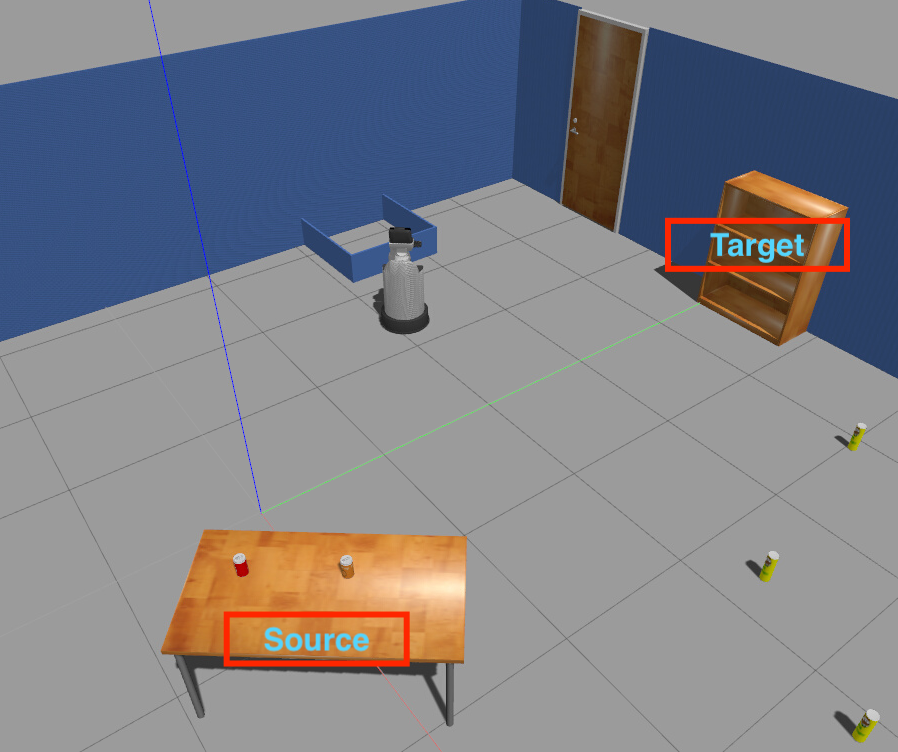
\includegraphics[width=0.8\textwidth]{pictures/knowledge/knowledge_roles_gr}
        \caption{Roles in Grocery Storing}
        \label{fig:kn_ro_gr}
    %\end{minipage}\hfill
    %\begin{minipage}{0.45\textwidth}
    %    \centering
        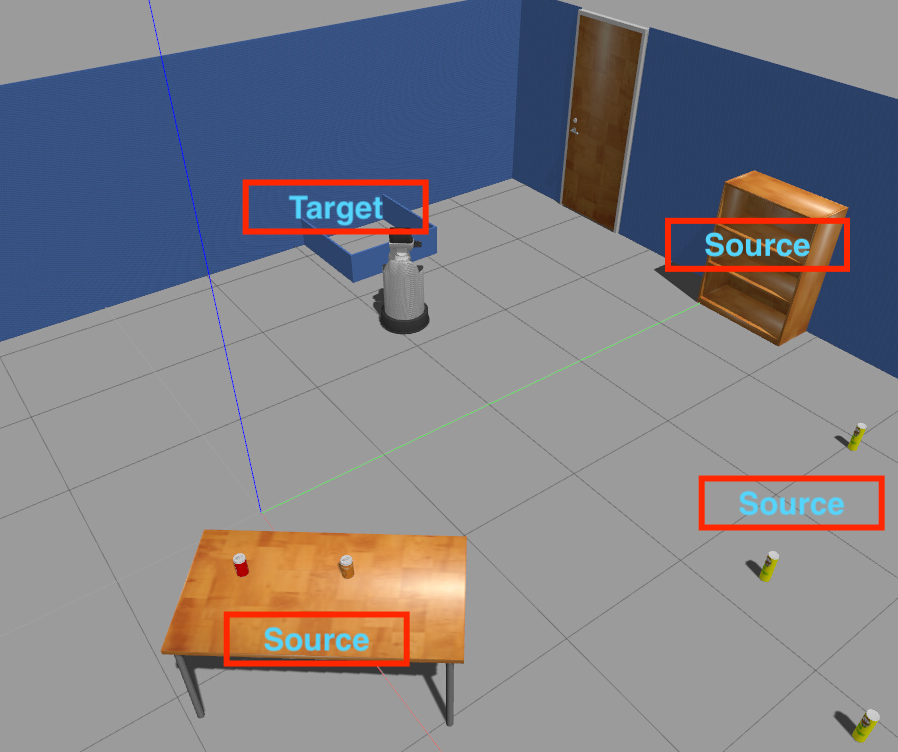
\includegraphics[width=0.8\textwidth]{pictures/knowledge/knowledge_roles_cl}
        \caption{Roles in Clean Up}
        \label{fig:kn_ro_cl}
    %\end{minipage}
\end{figure}

To be able to use the same predicates for both Tasks Grocery Storing and Cleanup, we implemented the concept of a surface role. All the most important predicates do something at a surface, depending on its role. For example, when we find the next object to grasp, it should be the next object standing on a surface, that we want to grasp from. Or when we place an object on a surface, it should be a surface that we want to put things on. Which surfaces get what role only depends on the task that the robot is currently working on. In the Grocery Storing task, all the shelves are target surfaces and all the tables are source surfaces (see figure \ref{fig:kn_ro_gr}), in the Cleanup task only the basket is a target surface and everything else (including the ground) is a source surface (see figure \ref{fig:kn_ro_cl}). This way, Knowledge doesn't need to know the specific task, it just needs to know, which surfaces have what role.\\
This is implemented by 

\begin{lstlisting}
make_role(SurfaceLink, Role):-
    rdf_retractall(SurfaceLink, hsr_objects:'sourceOrTarget',_),
    rdf_assert(SurfaceLink, hsr_objects:'sourceOrTarget', Role).
\end{lstlisting}
and there are a few other predicates, that use this \textit{make\_role/2} and apply it to different lists of surfaces:
\begin{lstlisting}
% Gives a list of surfaces the role source
make_surfaces_source(Surfaces):-

% Gives a list of surfaces the role target
make_surfaces_target(Surfaces):-

% Gives all surfaces with given name (ground, table, basket or shelf) the Role (target or source)
make_all_surface_type_role(SurfaceType, Role):-
\end{lstlisting}


\subsection{spatial\_comp.pl}

In the \textit{spatial\_comp} module are all the predicates, that help calculating something. Most importantly this includes the predicates, that can tell, on which surface a specific object is standing on or a specific position would be above. This helps us to map the objects to the surfaces and to double-check, if a calculated goal position for an object is valid. This is done by the two predicates

\begin{lstlisting}
% finds and returns surfaces the object might be standing on.
object_supportable_by_surface(Object, Surface):-

position_supportable_by_surface(Position, Surface) :-
\end{lstlisting}

Also, this module contains the wildly used predicate to calculate the distance between an Object or a Surface to the robot:

\begin{lstlisting}
distance_to_robot(Thing, Distance) :-
\end{lstlisting}

\subsection{urdf.pl}

Surfaces and Objects both have two kinds of representation in Knowledge. Mostly Knowledge works with their link in the ontology and asserts and queries RDF Triples with them. But for some calculations it is helpful, to work with the TF Tree, too. For example to calculate distances, to get the position of an object in the world or the object position relative to the surface it is standing on etc.. This is where the \textit{urdf} module comes in handy. It is nothing more than a conversion module to get from one representation to the other.

\subsection{mocking.pl}

To make testing easy, the \textit{mocking} module simulates some data, that otherwise would be generated by other groups of SUTURO. With

\begin{lstlisting}
create_object_on_surface(Surface) :-
\end{lstlisting}

you can create an object at a random suitable position on the Surface you want to. 

With 

\begin{lstlisting}
% This simulates the behavior of an Object, that gets taken by the 
% Gripper and than released at a different place.
% i.e. it simulates the result of
% attach_object_to_gripper(Object),
% release_object_from_gripper([Translation, Rotation]).
mock_new_object_place(Object, [Translation, Rotation]) :-
\end{lstlisting}

you can assign an object to a new place as if it was taken by the robot and put somewhere else.

\section{Ontology}
\chapterauthor{Fabian Rosenstock}
\subsection{About Ontologies}
An Ontology is a knowledge representation. To fulfill this task ontologies define classes, their attributes, and relations between them. Ontologies are hierarchical build and different axioms and restrictions for classes can be defined.


\subsection{RoboCup}
The RoboCup ontology defines concepts used to describe the RoboCup and concepts needed for the URDFs. To do that it imports the \textit{srdl2-comp} ontology that is part of \textit{KnowRob}. Furthermore the \textit{objects} ontology gets imported.\\
Since the concept of the RoboCup is not fully implemented yet, this ontology does not contain much apart from a class for the RoboCup, the tasks Clean-up and Grocery Storing, and a \textit{supports} property, that connects an object to the objects it supports.

\subsection{Objects}

This ontology describes and categorizes different physical objects according to their properties or common uses. These categories help to reason over objects, for example, to find similar objects. The Ontology furthermore defines different properties objects can have. \\
The \textit{objects} ontology imports the \textit{KnowRob} and the URDF ontology provided by \textit{KnowRob}.\\
For the description of objects, different regions are defined. Classes that represent different colors are added in the objects ontology as subclasses of \textit{ColorRegion} and different materials are defined in subclasses of \textit{MaterialRegion}. Different shapes are represented by subclasses of \textit{ShapeRegion}. An overview over the regions is given in figure \ref{fig:region_ont}.

\begin{figure}
\centering
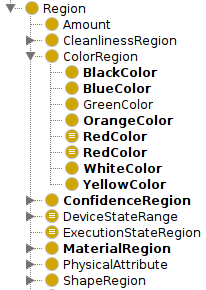
\includegraphics[width=1.0\textwidth]{pictures/ontology/Ontologie_region}
\caption{Regions}
\label{fig:region_ont}
\end{figure}

For those characteristics subclasses of \textit{PhysicalQuality} have been added, as seen in figure \ref{fig:quality_ont}.

\begin{figure}
\centering
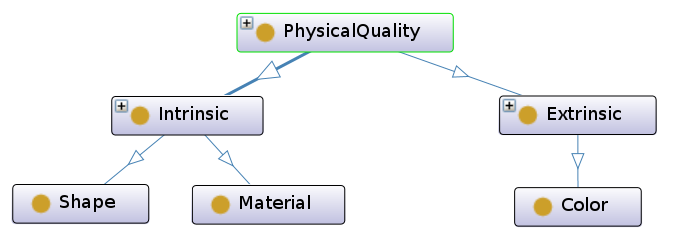
\includegraphics[width=1.0\textwidth]{pictures/ontology/Ontologie_quality}
\caption{Qualitys}
\label{fig:quality_ont}
\end{figure}

 Those represent the quality of the object, while the regions represent the actual values.\\
To represent the confidence with which the robot perceived a characteristic of an object the class \textit{ConfidenceRegion} and subclasses for the different characteristics are defined.\\
Physical objects are represented by the subclasses of \textit{PhysicalObject}.
One of these subclasses is \textit{PhysicalPlace}. The subclasses of \textit{PhysicalPlace} represent places, like the shelf. The surfaces are represented by subclasses of \textit{PhysicalPlace} as well. To represent this \textit{PhysicalPlace} has the subclass \textit{Surface}, where different kinds of surfaces are defined. This can be seen in figure \ref{fig:place_ont}.

\begin{figure}
\centering
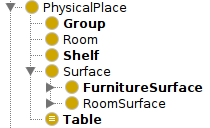
\includegraphics[width=1.0\textwidth]{pictures/ontology/Ontologie_place}
\caption{Physical places}
\label{fig:place_ont}
\end{figure}

The \textit{Unknown} class represents perceived objects, for which the robot doesn't know or is not sure what kind of physical object it is.\\
Most of the items, that have a representation in the \textit{objects} ontology, are subclasses of \textit{DesignedArtifact}.
Here you can find every item, that is created following a certain design. 
Examples for this are \textit{DesignedFurniture} like a table and \textit{DesignedTools} like a knife.\\
A huge part of the known items is different kinds of food or drinks. Most of these are categorised as \textit{ProcessedFood} or \textit{Drink}. Both of these are a subclass of \textit{DesignedSubstance}. The exception to this is things like tomatoes since these are not designed and therefore don't fit in the \textit{DesignedArtifact} class. Those objects are categorised as \textit{NaturalFood}, a subclass of \textit{BiologicalObject}. This class is a subclass of \textit{PhysicalBody}. The figure \ref{fig:object_ont} gives an overview over the \textit{PhysicalObject} class.

\begin{rotatepage}
\begin{figure}[H]
\centering
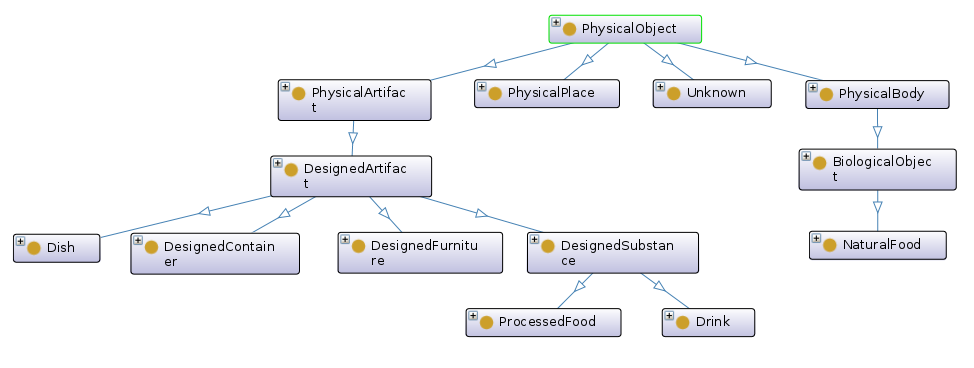
\includegraphics[width=1.5\linewidth, angle=90]{pictures/ontology/Ontologie_objects}
\caption{Physical objects}
\label{fig:object_ont}
\end{figure}
\end{rotatepage}

The object properties \textit{hassurface} and \textit{issurfaceof} are used to connect a surface and the dedicated object.\\
Since these surfaces can fullfill different roles the properties \textit{hasLocationRole} and \textit{isLocationRoleOf} are defined to connect the \textit{Source} and \textit{Target} roles to surfaces.\\
For the grouping of objects, the property \textit{inGroup} is responsible. This property connects an object to a group.\\
The \textit{supportedBy} property connects an object to the object (most likely surface) it is standing on.\\
To store the confidence for the different characteristics, sub-properties of the property \textit{hasRegionDataValue} have been added.\\
The \textit{size} property is responsible for storing the size of an object.\\
To distinguish objects the robot can move from others the \textit{supportable} property has been added. This property stores a boolean for an object.



\section{Scripts and higher Architecture}
\chapterauthor{Fabian Rosenstock}	  	
\subsection{store\_object\_info\_server.py}
This script stores the send data in the Knowledge base.
To do that it first checks if the class name is empty. Furthermore, the script changes the name of the class if it is not empty since Perception uses different naming conventions. After that, it tests whether the class exists in the \textit{objects} ontology. If the class name is empty or if the class does not exist in the \textit{objects} ontology the class gets changed to the generic other class. Then all the information on the object get extracted out of the \textit{ObjectDetectionData} message. If the object has a legal position it gets added to the Knowledgebase and the objects at that position are put into one group.

	\endgroup

\end{document}


